\newcommand{\nc}[0]{n_{\mathrm{c}}}
\newcommand{\todo}[1]{{\color{red} [#1]}}

\chapter{\label{ch:4-aggregation}\chaggregation}

\minitoc
% \newpage

\section{Background}

Protein-protein interactions, while crucial for normal cellular function, can also be the underlying cause of disease. This can occur in two main ways: (a) by interfering with the proteins' normal function, or (b) by causing proteins to adopt a toxic mode of action. A notable example of this is found in diseases associated with protein aggregation. In these conditions, proteins aggregate into large, typically linear structures known as fibrils, where multiple monomer proteins combine in an ordered fashion \cite{chiti_protein_2006}.


\todo{Somehow link the misfolding aspect in..? and the free energy landscape etc.}

These aggregates can contribute to disease through both mechanisms mentioned: (a) by sequestering functional proteins, thereby reducing the concentration of free monomers available for normal cellular functions, and (b) by producing reactive, toxic oligomers that harm the cell. \cite{chiti_protein_2006, chiti_protein_2017} Oligomers are small, partially structured protein aggregates that serve as intermediaries in the formation of fibrils. These oligomers can undergo internal structural reorganisation, forming short, ordered aggregates that then attract additional monomers, eventually maturing into long fibrils composed of thousands of monomers. The toxicity of oligomers is primarily driven by two factors: their exposed hydrophobic groups and their high reactivity. The latter is due to the shallow energy well in the oligomers' structural free energy landscape, which makes them highly reactive. Additionally, their small size enables them to diffuse rapidly, allowing them to thoroughly explore the cellular environment and disrupt various cellular processes.


\todo{dont know the exact mechanisms of toxicity but think its all...}


\cite{chiti_protein_2017}


\subsection{Aggregating Neurodegeneartive Disease}

Protein aggregation that occurs in the brain is called neurodegenerative diseases. These inlcude a wide variety of 

Need to intro acronyms, NDDs, AD, PD, ALS
some examples include Alzheimers Disease, Parkinson's Disease, Huntingtons's Disease, amyotrophic lateral sclerosis (ALS)

\section{Aggregation Kinetics in vitro}

There are multiple processes that can convert single protein monomers into ordered aggregates. We model these aggregates as 1D chains of the monomer protein which can vary in length and describe an aggregate of length $i$ as $\mathcal{A}_i$, and the concentration of aggregates of size $i$ is given by $p_i$. We describe the monomers as $\mathcal{M}$ and the monomer concentration as $m$. There are typically three distinct mechanisms that can form new aggregates:
\begin{itemize}
    \item \textbf{Primary Nucleation} is the spontaneous conversion of $\nc$ monomers into an aggregate of length of $\nc$: $\nc\mathcal{M} \rightarrow \mathcal{A}_{\nc}$. Using mass action, we expect the rate of this reaction to be $k_n m^{\nc}$ where $k_n$ is the rate constant for this process. We expect that $\nc$ is set by the energy dependence on aggregate length and so $\nc$ is constant and all aggregates smaller than $\nc$ are unstable and subsequently ignored.
    \item \textbf{Secondary Nucleation} is the conversion of $n_2$ monomers into an aggregate of length of $n_2$ occurring on the surface of existing aggregates: $n_2 \mathcal{M} + \mathcal{A}_{i} \rightarrow \mathcal{A}_{n_2} + \mathcal{A}_{i}$. This reaction occurs uniformly over the surface (i.e. length) of all existing aggregates and so we expect the rate to be proportional to the total length of aggregates, $\sum i p_i$. The reaction rate then becomes $k_2 m^{n_2}(\sum i p_i)$ where $k_2$ is the rate constant for secondary nucleation.
    \item \textbf{Fragmentation} is the splitting of a longer aggregate into two smaller aggregates: $\mathcal{A}_{i+j} \rightarrow \mathcal{A}_{i} + \mathcal{A}_{j}$. Again, we assume that fracturing occurs uniformly over every bond between monomers, so that for an aggregate of size $i$, there are $i-1$ bonds that could fracture. The rate for a specific bond to fracture will be some constant rate, $k_{-}$, however the overall fracture rate of aggregates of size $i$ will be $k_{-}(i-1)p_i$. When an aggregate fractures it two new smaller aggregates and so increases the number of aggregates.
\end{itemize}

\begin{figure}
    \centering
    \includegraphics[width=0.8\textwidth]{figures/4-agg-figs/aggProcesses.pdf}
    \caption{Aggregation Processes.}
    \label{fig:4-phase_sep_scheme}
\end{figure}

\noindent Additionally, aggregates changes size via the addition or removal of a monomer protein on the end of an aggregate, we describe this process as:
\begin{itemize}
    \item \textbf{Elongation} The addition of a monomer onto an existing aggregate: $\mathcal{M} + \mathcal{A}_{i} \rightarrow \mathcal{A}_{i+1}$. This happens at rate $2 k_\text{on} m \sum p_i$
    \item \textbf{Depolymerisation} The dissociation of a monomer from an existing aggregate: $\mathcal{A}_{i} \rightarrow \mathcal{M} + \mathcal{A}_{i-1}$. Since the addition of a monomer can happen at either end of the aggregate, the elongation happens at a rate $2 k_{off} \sum p_i$.
\end{itemize}

This gives the master equation that describes the evolution of the population of aggregates of a given length $i$, 
\begin{equation}
\begin{split}
    \frac{\text{d}p_i}{\text{d}t} &= \delta_{i, n_C}k_n m^{n_C} + \delta_{i, n_2} k_2 m^{n_2} \left(\sum_{j=\nc}^{\infty} j p_j\right) + 2k_\text{on} m (p_{i-1}-p_i) \\
    & + 2k_{off} (p_{i+1}-p_i) - k_{-}(i-1)p_i + 2k_{-}\left(\sum_{j=i+1}^{\infty}p_j\right).
    \end{split}
    \label{eq:4-pi_evolution}
\end{equation}
The final term that describes the rate at which new aggregates are made has an additional factor of $2$. This is because an aggregate of length $j>i$ can split at two different points to form an aggregate of length $i$, either at the $i^{\text{th}}$ or $(j-i)^{\text{th}}$ monomer. Exceptionally, when $j=2i$ there is only one place where the aggregate can break to produce aggregates of length $i$, however this produces two aggregates of length $i$, $\mathcal{A}_{2i}\rightarrow2\mathcal{A}_i$, and so the rate maintains the factor two. In general, this infinite system of coupled ordinary differential equations is hard to solve. Strategies to numerically integrate the system involve truncating the series of $p_i$s and introducing some boundary conditions in the length space, e.g. introducing an absorbing boundary by setting the population of very larger aggregates to be zero.
\todo{Justifiy ingnoring fragmentation/why it can be written as in Georg's thesis?}

Experimental methods \todo{such as...} often measure the total mass of bound protein, that is
\begin{equation}
    M = \sum_{i=\nc}^{\infty}i p_i.
\end{equation}
This defines the second moment of the $p_i$ distribution and we can also define the first moment, $P$, as 
\begin{equation}
    P = \sum_{i=\nc}^{\infty} p_i.
\end{equation}
which is simply the number of aggregates. Summing over the master equation (or differentiating $M$), we can find the evolution of these moments from the master equation and \todo{for the no fragmentation case} we find that these form a closed system of equations
\begin{align}
    \frac{\text{d}M}{\text{d}t} &= 2 k_\text{on}m P + \nc k_n m^{\nc}+ k_2 m^{n_2} M, \label{eq:4-Mvitro} \\
    \frac{\text{d}P}{\text{d}t} &= k_n m^{n_c}+k_2 m^{n_2} M. \label{eq:4-Pvitro}
\end{align}
To fully close the system we also need to consider the monomer concentration. In test tube experiments, there is a fixed quantity of monomer that is converted into aggregates. The total protein in an experiment is constant, $M_{total} = M + m$, so that $\dot{m}=-\dot{M}$ (where the dot is a derivative with respect to time). For completeness we write this explicitly as 
\begin{equation}
    \frac{\text{d}m}{\text{d}t} = -2 k_\text{on}m P - 2k_n m^{n_c} - 2k_2 m^{n_2} M. \label{eq:4-mvitro}
\end{equation}
Standard numerical solvers can integrate this closed system of equations to determine the \textit{aggregation curve} that describes the transition from monomer to aggregate. Fitting this solution to aggregation data shows an extremely good fit and can be used to determine the rate constants of aggregation, e.g. $k_\text{on}$, $k_2$ etc.

\begin{figure}
    \centering
    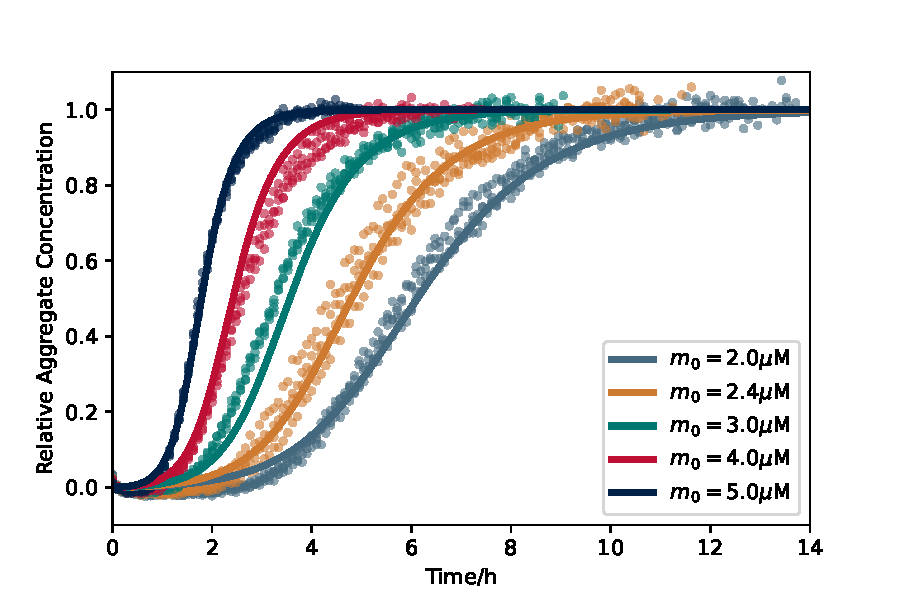
\includegraphics[width=0.8\textwidth]{figures/4-agg-figs/invitroDemo.pdf}
    \caption{Fitting in vitro aggregation data. The rate constants have been fit globally. We set $\nc=2$, $n_2=2$ and fit $k_on k_2=5.60\times10^{16}$ and $k_on k_n=9.992\times10^{8}$}. Fitting has been done using \textit{AmyloFit} software \cite{meisl_molecular_2016}. Data taken from \cite{cohen_proliferation_2013}.
    \label{fig:4-invitro}
\end{figure}

\todo{Mention how we can actually get the aggregation data perhaps?} Typical aggregation have an initial exponential increase in aggregate concentration due to the secondary nucleation process. As the monomer concentration is depleted the rate of aggreagtion slows until all the monomer is aggregated. The secondary nucleation step is autocatalytic as aggregates speed up the formation of more aggregates leading to a postive feedback and fast transition from mostly monomer to mostly aggregate.\todo{Discussion of scaling, typical length, etc., could actually also plot M/P, but just generally could have a bit more discussion here.}

\subsection{Failure to Recapitulate Disease}

The aggregation curves in test tube experiments are well understood by the reaction kinetics, but lack many crucial features of the development of neurodegenerative disease in living systems. Specifically, the model in (\ref{eq:4-Mvitro})-(\ref{eq:4-mvitro}) does recapitulate the discrete seeding transition, observed recovery of mice following treatment, or explain why the disease typically occurs in later life. These observations and the contradiction with the in vitro model are outlined below.

\subsubsection{Discrete seeding transition to disease}

In some model systems of neurodegenerative diseases, aggregation is only observed when the tissue or cells are seeded \cite{miller_tau_2021, tuck_cholesterol_2022}. For example, pathological aggregates are only observed in hippocampal slice cultures from P301S tau transgenic mice when the system is exposed to a high concentration of preformed assemblies at some earlier time (seeding) \cite{miller_tau_2021}. Small doses of tau assemblies do not increase aggregate concentration when compared to an unseeded system. However, for large doses of tau assemblies, the observed aggregate concentration was increased (and further increased when the dose was increased again). This phenomena is well established \cite{jucker_propagation_2018} and has been used to develop reporter lines assays to determine the presence of aggregates.\todo{cite the reporter}

The in vitro dynamics cannot explain this phenomena. The in vitro early time aggregation is dominated by an exponential growth, from the secondary nucleation process, $M(t) = M_0\exp(k_2 m_0^{n_2}t)$ where $M_0$ is the aggregate population at time $t=0$. Thus, addition of a seeding mass of aggregates, $M_S$, would correspond to shifting the aggregation process in time, but would not cause this transition between a stable and unstable system at some non-zero seeding.

% At early time in the in vitro dynamics, the aggreagtes proliferate exponentially. Thus, an injection of seed concentration acts to speed up this aggreagation process and can lead to much highe concntrations. However, this cannot describe the situation in all systems, as the . Additionally, when the seed concentration is varied, this exponential hypothesis would predict that the observed aggregate


% An existing hypothesis surrounding the onset of diseases from protein aggregation are built around the early time exponential growth of the disease. Specifically, that 
% The exponential growth hypothesis predicts that aggregate mass increases exponentially in time
% \begin{equation}
%     M(t) = S\exp{\kappa t}
% \end{equation}
% where $S$ is the aggregate mass at time $t=0$. In a seeded system, we typically expect the seeded aggregate mass to be much greater than the natural mass of aggregates and so we approximate $S$ as the mass of seeds.

% Consider three identical systems, seeded with different initial concentrations of the aggregated proteins; $S_1$, $S_2$, and $S_3$. The systems will aggregate and at some threshold, $M_D$, we will detect the aggregates in the cell. The exponential growth hypothesis can be used to identify growth rates. We identify the first time that aggregates are seen at as $t_i$ for a system seeded with $S_i$ aggregates. Then the growth rate, $\lambda$, is given by
% \begin{equation}
%     \lambda = \frac{\ln(S_1)-\ln(S_2)}{t_2-t_1}
% \end{equation}
% Therefore an experiment that does not satisfy this
\subsubsection{Explaining and Informing Treatments}

Currently the leading therapeutics for neurodegenerative diseases are based on immune therapies, such as monoclonal antibody therapies. In these treatments, antibodies bind to pathological fibrils to either disrupt the toxicity, or identify the structures for destruction via immune processes \cite{wisniewski_immunotherapeutic_2015, berg_biochemistry_2002}. \todo{list some current therapies?} These processes do not occur in test tubes and so cannot be described or explored by in vitro models.

More recently, short, synthetic, single-stranded DNA or RNA molecules, called antisense oligonucleotides (ASOs) are being explored as therapeutic candidates to treat NDDs \cite{rinaldi_antisense_2018}. The ASOs bind to target mRNA and thus limit transcription, reducing the expression of the aggregating monomer protein. In multiple studies, injections of ASOs were able to reduce the monomeric protein and this led to reduction and even removal of aggregates in the brain \cite{cole_-synuclein_2021, devos_tau_2017, mummery_tau-targeting_2023}. These studies demonstrate the enormous clinical potential of ASOs that target tau and $\alpha$-synuclein, two aggregating proteins associated with PD and AD. This presents a major opportunity to develop effective treatments for NDDs.

However, in order to realise these therapeutic opportunities, it is necessary to understand the different processes that affect the development of the disease in living cells and tissues. Test tube experiments show an inevitable conversion of monomer into aggregates, and cannot recapitulate the behaviour responsible for the reduction of aggregates and associated recovery of brain function in treated mice \cite{cole_-synuclein_2021}. Furthermore, developing a quantitative theory that can describe the onset and progression of disease will resolve the size of effects required for an intervention to have a meaningful change in prognosis.

\subsubsection{Long timescale in disease}\label{subsubsec:onsetage}

Test tube aggregation kinetics provide estimations for typical aggregation parameters and timescales. Typical aggregation experiments, such as those shown in Figure \ref{fig:4-invitro}, approach completion after around 10 hours, and have a doubling time of around an hour during the early exponential growth phase \cite{meisl_mechanistic_2022}. However, this understanding does not translate to the onset of disease in human populations. Around one in ten adults over the age of 65 have AD, increasing to four in every ten adults over 95 \cite{hou_ageing_2019}. This late age of onset is also seen for PD and ALS, with only $4\%$ of PD cases being under the age of 50 and the incidence increasing by a factor of $5$–$10$ from cases in their fifties to eighties \cite{van_den_eeden_incidence_2003, poewe_parkinson_2017}. This disparity of five orders of magnitude (one hour to one decade) clearly shows that something is missing from the current mechanistic models mapping in vitro protein aggregation kinetics onto the development of disease. In this chapter I will identify processes that are missing in vitro and develop a model to include all of these competing mechanisms. I will then demonstrate how these models can explain previously inexplicable observations and the consequences for the design of rational therapeutics.

\section{Aggregation Kinetics in vivo}

In living systems, there are additional processes in the `life cycle' of a protein. Specifically, how proteins are manufactured and removed. Many proteins that aggregate during disease are functional, for example \todo{specifics}. As such, we expect the concentration of these proteins will be maintained as part of homeostasis and thus in vivo the monomer concentration is constant, $m(t)=m_0$. In order to maintain the monomer concentration precisely, the cellular production and removal will need to be much faster than the aggregation kinetics and thus we write this as
\begin{equation}
    \frac{\text{d}m}{\text{d}t} = \epsilon^{-1}\left( \gamma - \lambda_1 m \right) + \text{aggregation kinetics}
    \label{eq:4-minvivo}
\end{equation}
where $\gamma$ and $\lambda_1$ are scaled rate constants for production and removal of the monomer respectively and $\epsilon$ is a small parameter that separates the timescales. The leading order solution to (\ref{eq:4-minvivo}) is $m=\gamma/\lambda_1$ which sets $m_0$. In the subsequent analysis we only consider this leading order behaviour. A full solution as an expansion of $\epsilon$ could be explored, however the leading order behaviour is sufficient to capture key features of the disease.

In living systems aggregates can also be removed via active processes in the cells or surrounding tissue. Examples of such processes include \todo{give examples}. This changes the master equation to
\begin{equation}
\begin{split}
    \frac{\text{d}p_i}{\text{d}t} &= \delta_{i, n_C}k_n m^{n_C} + \delta_{i, n_2} k_2 m^{n_2} \left(\sum_{j=\nc}^{\infty} j p_j\right) + 2k_\text{on} m (p_{i-1}-p_i) + 2k_{off} (p_{i+1}-p_i) - \lambda_i(p_i),
    \end{split}
    \label{eq:4-pi_cleared}
\end{equation}
where $\lambda_i(p_i)$ is the clearance rate for aggregates of each size.

\subsection{Unbounded Clearance}

The exact mechanisms of clearance and their kinetics remain unknown in many living systems. In the spirit of Occam's (or informally OCIAM's) razor we begin by considering the simplest kinetics: the clearance rate is proportional to the number of aggregates and independent of size $\lambda_i(p_i)=\lambda \times p_i$. We begin by analysing this system to demonstrate the inability to recapitulate all observed experimental results and to build an analysis framework for other systems.


The moment equations now define a linear system, since $m=m_0$ is constant, and so we can define $\textbf{q}=(P, M)^\text{T}$ and the evolution of the system becomes
\begin{equation}
    \dot{\textbf{q}} =
    \underbrace{\left(
    \begin{array}{cc}
    -\lambda & k_2 m_0^{n_2} \\
    2 k_\text{on}m_0 & n_2 k_2 m_0^{n_2}-\lambda  \\
    \end{array}
    \right)}
    _{\textbf{A}}
    \textbf{q}
    +
    \underbrace{\left(
    \begin{array}{c}
    k_n m_0^{\nc} \\
    \nc k_n m_0^{\nc} \\
    \end{array}
    \right)}
    _{\textbf{b}}
    \label{eq:4-momentEvomatform}
\end{equation}
where the dot indicates the time derivative and we've defined the matrix $\textbf{A}$ and vector ${\textbf{b}}$ in the equation. The solution is 
\begin{equation}
    \textbf{q} = -\textbf{A}^{-1}\textbf{b}+\left(\textbf{q}_0+\textbf{A}^{-1}\textbf{b}\right)e^{\textbf{A}t}
    \label{eq:4-momentSolvematform}
\end{equation}
where $\textbf{q}_0$ is a vector of the initial aggregate number and aggregate mass concentration. The steady state behaviour is determined by the eigenvalues of $\textbf{A}$, which are
\begin{equation}
    \nu_{\pm} = \frac{1}{2} \left(k_2 m_0^{n_2} n_2 \pm \sqrt{8 k_\text{on} m_0 k_2 m_0^{n_2} + \left(n_2 k_2 m_0^{n_2}\right)^2} - 2 \lambda \right).
    \label{eq:4-A_eig}
\end{equation}
The system always has $\nu_{-} \leq 0$, however the sign of $\nu_+$ depends on the the clearance constant, $\lambda$. If $\nu_+>0$, then the system has no steady state and both the mass and number of aggregates has unbound growth. For $\nu_+<0$ then there exists a steady state solution for $t\rightarrow\infty$, $\textbf{q}_\infty = -\textbf{A}^{-1}\textbf{b}$. The stability of the system is independent of the primary nucleation rate as there is no positive feedback on the production of aggregates, however this nucleation process still affects the steady state aggregate mass. Given a set of rate constants we can therefore define a \textit{critical clearance}, $\lambda_{\text{crit}}$, that determines whether the aggregation will be bound. Solving equation (\ref{eq:4-A_eig}) for $\nu_+=0$ gives
\begin{equation}
    \lambda_{\text{crit}} = \frac{1}{2} \left(k_2 m_0^{n_2} n_2 + \sqrt{8 k_\text{on} m_0 k_2 m_0^{n_2} + \left(n_2 k_2 m_0^{n_2}\right)^2}\right).
    \label{eq:2-critclear}
\end{equation}
\todo{check this critical value} When $\lambda>\lambda_{\text{crit}}$ the system approaches a steady state and when $\lambda<\lambda_{\text{crit}}$ the mass of aggregates grows exponentially as $M(t)\sim M(0)e^{\nu_+ t}$.

Alternatively, we could fix the clearance rate and determine the maximum monomer concentration, $m_0$, that leads to a steady state solution. The stability condition is
\begin{equation}
    -2 k_2 k_\text{on} m_0^{n_2+1} - n_2 k_2 \lambda m_0^{n_2} +\lambda^2 = 0
    \label{eq:2-critmon}
\end{equation}
which has exactly one positive solution that defines the critical monomer concentration $m_0^{(crit)}$. At monomer concentrations above $m_0^{(crit)}$ the system has unbound aggregation and below $m_0^{(crit)}$ the aggregate mass approaches a steady state. This is a useful perspective as the new treatment technologies, such as ASO/CHARM treatments can vary $m_0$ as a therapeutic strategy, however currently no theoretical description exists to capture this.

At the steady state, $\textbf{q}$ is constant, and so we can determine the average aggregate length as the ratio of the aggregate mass and aggregate number, $\bar{l}=P/M$. At the steady state this will be constant
\begin{equation}
    \bar{l}^* = \frac{M^*}{P^*} = \frac{2 k_\text{on} m_0 + \nc \lambda_{\text{crit}}}{\lambda_{\text{crit}}+(\nc-n_2)k_2 m_0^{n_2}}.
    \label{eq:4-lbarConstClear}
\end{equation}
The effect of secondary nucleation on the average length initially seems confusing, and in particular it might seem strange that the dependence on $k_2$ vanishes when $\nc=n_2$. This can be explained as aggregates are only nucleated at length $\nc$ or $n_2$ and the population of aggregates at other lengths decays geometrically away from these source terms. When $\nc = n_2$ there is only one source term, therefore the average aggregate length is determined entirely by the rate of decay of the aggregate population with increasing length. If the nucleation rate were increased, the population at length $n_c$ would increase, and subsequently the population of aggregates of every length would increase proportionally, however the decay length would remain the same and the \textit{average} aggregate length would also be unchanged. For $n_2>\nc$ the source term at $n_2$ increases the aggregate population at large lengths and so increases the average length.

\subsubsection{Exactly Solving the Full Linear System}

When the system clears aggregates at a linear rate we can calculate the steady state aggregate length distribution as well as the time evolution of an arbitrary number of moments of this distribution.

Additionally, we can determine the time full evolution of any initial distribution in the moment space. Since this is a linear system, the we can take an arbitrary number of moments. Define
\begin{equation}
    Q^{N} = \sum_{\nc}^\infty i^N p_i
\end{equation}
which has the time evolution
\begin{equation}
\begin{split}
    \frac{\text{d}Q^{N}}{\text{d}t} &= \sum_{\nc}^\infty i^N \left( \delta_{i, n_C}k_n m^{n_C} + \delta_{i, n_2} k_2 m^{n_2} M + 2k_\text{on} m (p_{i-1}-p_i) + 2k_{off} (p_{i+1}-p_i) - \lambda p_i \right) \\
    \frac{\text{d}Q^{N}}{\text{d}t} &= \sum_{\nc}^\infty i^N \left( \delta_{i, n_C}k_n m^{n_C} + \delta_{i, n_2} k_2 m^{n_2} M + 2k_\text{on} m (p_{i-1}-p_i) - \lambda p_i \right) \\
    &=n_C^N k_n m^{n_C} + n_2^N k_2 m^{n_2} M + \sum_{\tau=0}^{N-1} 2k_\text{on} m \binom{N}{\tau} Q^{\tau} - \lambda Q^{N}.
\end{split}
\end{equation}
Since the evolution of a moment only depends on itself, or moments of lower order moments, we can still solve the system equation (\ref{eq:4-momentEvomatform}).

It is also possible to find $p_i$ for the steady state. Assume $n_c=n_2$. In steady state the concentration of each aggregate size is in detailed balance so for the smallest aggregates, of length $n_c$, we have
\begin{equation}
    k_n m_0^{\nc} + k_2 m_0^{\nc} M - 2 k_\text{on} m_0 p_{\nc} - \lambda p_{\nc} = 0
    \label{mpnc1}
\end{equation}
and detailed balance for all aggregates of other lengths gives
\begin{equation}
    (2k_\text{on} m_0 + \lambda)p_{i+1} = 2k_\text{on} m_0 p_i.
\end{equation}
This is solved by
\begin{equation}
    p_i = \alpha^{i-\nc} p_{\nc}\quad\text{ with }\quad\alpha=\frac{2k_\text{on} m_0}{2k_\text{on} m_0 + \lambda}
\end{equation}
and so we get another equation connecting $M$ and $p_{\nc}$, that is
\begin{equation}
    M = \sum_{i=\nc}^{\infty}i\alpha^{i-\nc} p_{\nc} = p_{\nc}\left( \frac{(\lambda +2k_\text{on} m_0) (2 k_\text{on} m_0 + \lambda  \nc)}{\lambda^2} \right).
    \label{mpnc2}
\end{equation}
Combining equations (\ref{mpnc1}) and (\ref{mpnc2}) gives the same mass, $M$, as before and 
\begin{equation}
    p_{\nc} = \frac{\lambda^2 k_n m_0^{\nc} }{(2 k_\text{on} m_0+\lambda \nc) \left(\lambda ^2-k_2 m_0^{\nc} (2 k_\text{on} m_0+\lambda  \nc)\right)}
\end{equation}
which for realistic signs of the parameters (e.g. no negative clearance) gives the critical behaviour at the same values as before. \todo{need to watch the bound for the $k_{off}$ term!}

Moving from the master equation to the moment description of the kinetics, we have assumed \todo{SC III: what assumptions have we made?}. Numerical simulation of the dynamics of the system at the level of the master equation can verify that the coarse grained description provides an accurate summary and prediction of the kinetics. In the most general case however, this presents computational challenges, as there is no upper limit on the aggregate length. Here, we introduce a maximum aggregate length that does not elongate but is still removed via the clearance mechanisms. The maximum length should be significantly larger than the mean length distribution and we can additional ensure that it is larger than lowest length populated by one aggregate, using equation \todo{get the equation in}. We then evolve this system using a \todo{fouth order Runge–Kutta method} to simulate the evolution of the full population distribution of aggregates of different lengths. \todo{Shows good agreement etc.?}

\begin{figure}
    \centering
    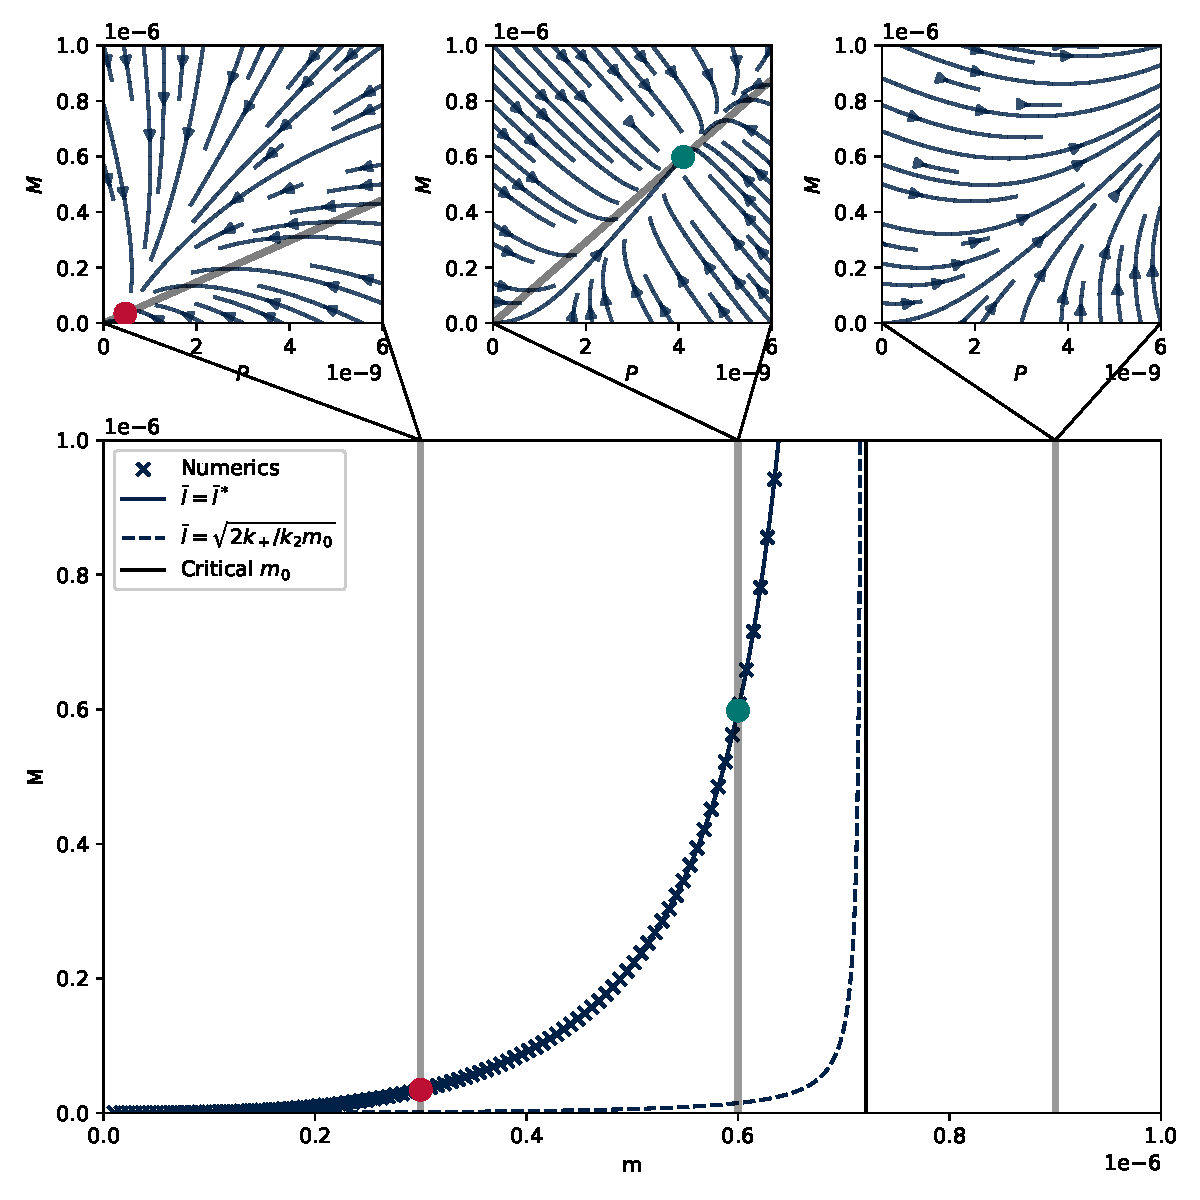
\includegraphics[width=0.8\textwidth]{figures/4-agg-figs/propClearSummary.pdf}
    \caption{Comparison of the different descriptions of the system, its flow and stability.}
    \label{fig:4-steadyConstClear}
\end{figure}

\subsection{Bounded Clearance}\label{subsec:4-boundedclearance}

The proportional clearance described above permits an analytically solvable model that gives insight into the role of clearance in neurodegenerative diseases. However the proportional clearance is an unphysical description for the removal of aggregates in all scenarios. Breaking down aggregates into the clearance products will require energy to break the bonds \todo{specify the bond} that connect the monomers and so the energy consumption rate will increase linearly with the rate of mass clearance. There will be some maximum energy consumption rate for the cell and this will therefore translate to a maximum clearance rate of aggregates. In this section we explore to fundamentally different phenomena that arise from this bounded clearance.

The exact functional form describing the kinetics of aggregate clearance will determine how the clearance rate approaches this upper bound. For example, there could be a finite fuel component such as ATP that is depleted as that aggregates are cleared and limits the clearance rate, the aggregates may cause toxic damage to the cell and affect the efficiency of cellular processes or, as we will assume, the clearance mechanism has enzyme-like rate kinetics. Consider the ubiquitin (Ub)-proteasome system (UPS) that tags aggregates with Ub before the aggregates are unfolded and cleaved in the proteasome, or chaperone mediated autophagy (CMA) where chaperones delivered to lysosomes to be degraded \cite{ciechanover_degradation_2015} \todo{GM: Ulrich Hartl refs} Both of these clearance processes can be modelled as the binding of an essential clearance component (E), either Ub or the chaperone, before the bound complex is then removed from the system and the intermediary clearance component is released. For an aggregate $A_i$, with concentration $p_i$ and an clearance component $E$ with concentration $p_e$, the clearance reaction can be modelled as
\begin{equation}
        \ce{A_i + E <=>[$k_i^b$][$k_i^d$] C_i ->[$k^{c}_i$] E + Clearance Products} \label{eq:4-MM}
\end{equation}
where $k_i^b$ and $k_i^d$ are the binding and dissociation rates of the aggregate and intermediary component which and $k^{c}_i$ is the rate constant describing the removal of the aggregate. The intermediate clearance component binds to an aggregate of size $A_i$ to form a complex $C_i$, with concentration $c_i$, which can either dissociate or be broken down and cleared.

This setup is similar to the Michaelis–Menten (MM) description for reactions kinetics where the $E$ component is the enzyme. However here we have a series of different sized aggregates that all compete for the same component. We can calculate the expected rates in the system in the same way as the single substrate analysis: assume that the total $E$ component in the system is constant, $p_e^{T} = p_e + \sum_i c_i$, and that the aggregate binding is at equilibrium for all lengths, $k_i^b p_e p_i = k_i^d c_i$. These expressions give
\begin{equation}
    c_i = p_e^{T}\frac{k_i^b}{k_i^d}\left(\frac{p_i}{1+\sum_j p_j \frac{k_j^b}{k_j^d}}\right).
\end{equation}
The clearance of aggregates of size $i$ in the system is $\lambda_i = k_i^{c}c_i$. In general this will not reduce to a closed form pair of moment equations, however if we assume that the rates are independent of aggregate size, $k_i^{c}=k^{c}$, $k_i^{b}=k^{b}$ and $k_i^{d}=k^{d}$, then this reduces to the typical MM kinetics, as each all aggregates are effectively the same single substrate. This now gives the moment equations with modified clearance as
\begin{align}
    \frac{\text{d}M}{\text{d}t}&= \nc k_n m_0^{\nc} + n_2 k_2 m_0^{n_2} M + 2 k_\text{on} m_0 P - \frac{\lambda_M M}{K_M+P} \\
    \frac{\text{d}P}{\text{d}t}&= k_n m_0^{\nc} + k_2 m_0^{n_2} M - \frac{\lambda_{M} P}{K_M+P}.
    \label{eq:4-reducedMM}
\end{align}
where we have defined $\lambda_M = k^{c} p_e^T$ and $K_M = k^d/k^b$. When $P \ll K_M$, the clearance is proportional to the concentration as before, with an equivalent clearance rate of $\lambda = \lambda_M/K_M$. However for $P \gg K_M$, the clearance saturates with a maximum number clearance rate $\lambda_M$ and a maximum mass clearance rate mass clearance rate $\lambda_M\bar{l}$.

Solving for the steady state of the system, $\text{d}M/\text{d}t=\text{d}P/\text{d}t=0$, gives three pairs of solutions for $M^*$ and $P^*$. For typical system parameters, two pairs of the steady states have real positive solutions for both $M^*$ and $P^*$. At a critical monomer concentration these two solutions undergo a bifurcation and merge, such that for monomer concentrations above this critical value there no longer exists a positive steady state. Similarly to the case for proportional clearance, when the monomer concentration is large we expect the mass of aggregates in a system to exhibit unbound growth. When the monomer concentration is less than this critical value, there exists a steady state, however unlike when the clearance is proportional, the system will not necessarily converge to this equilibrium. Whether the steady state is reached depends on the initial mass and number concentrations ($M$ and $P$).

Again, we can solve for the steady state length distribution when this exists. For $\nc=n_2$ we have
\begin{equation}
    k_n m_0^{\nc} + k_2 m_0^{\nc} M - 2 k_\text{on} m_0 p_{\nc} - \frac{\lambda_P p_{\nc}}{K_M + P} = 0
\end{equation}
and detailed balance for all aggregates of other lengths gives the same geometric decay, but with a different decay rate, $\alpha$,
\begin{equation}
    p_i = \alpha^{\nc-i} p_{\nc}\quad\text{ with }\quad\alpha=\frac{2k_\text{on} m_0 (K_M + P)}{2k_\text{on} m_0 (K_M + P) + \lambda_P}.
\end{equation}
Evaluating the sums to determine $M$, $P$ and $p_{\nc}$, gives the same pair of positive real solutions, as expected.

\begin{figure}
    \centering
    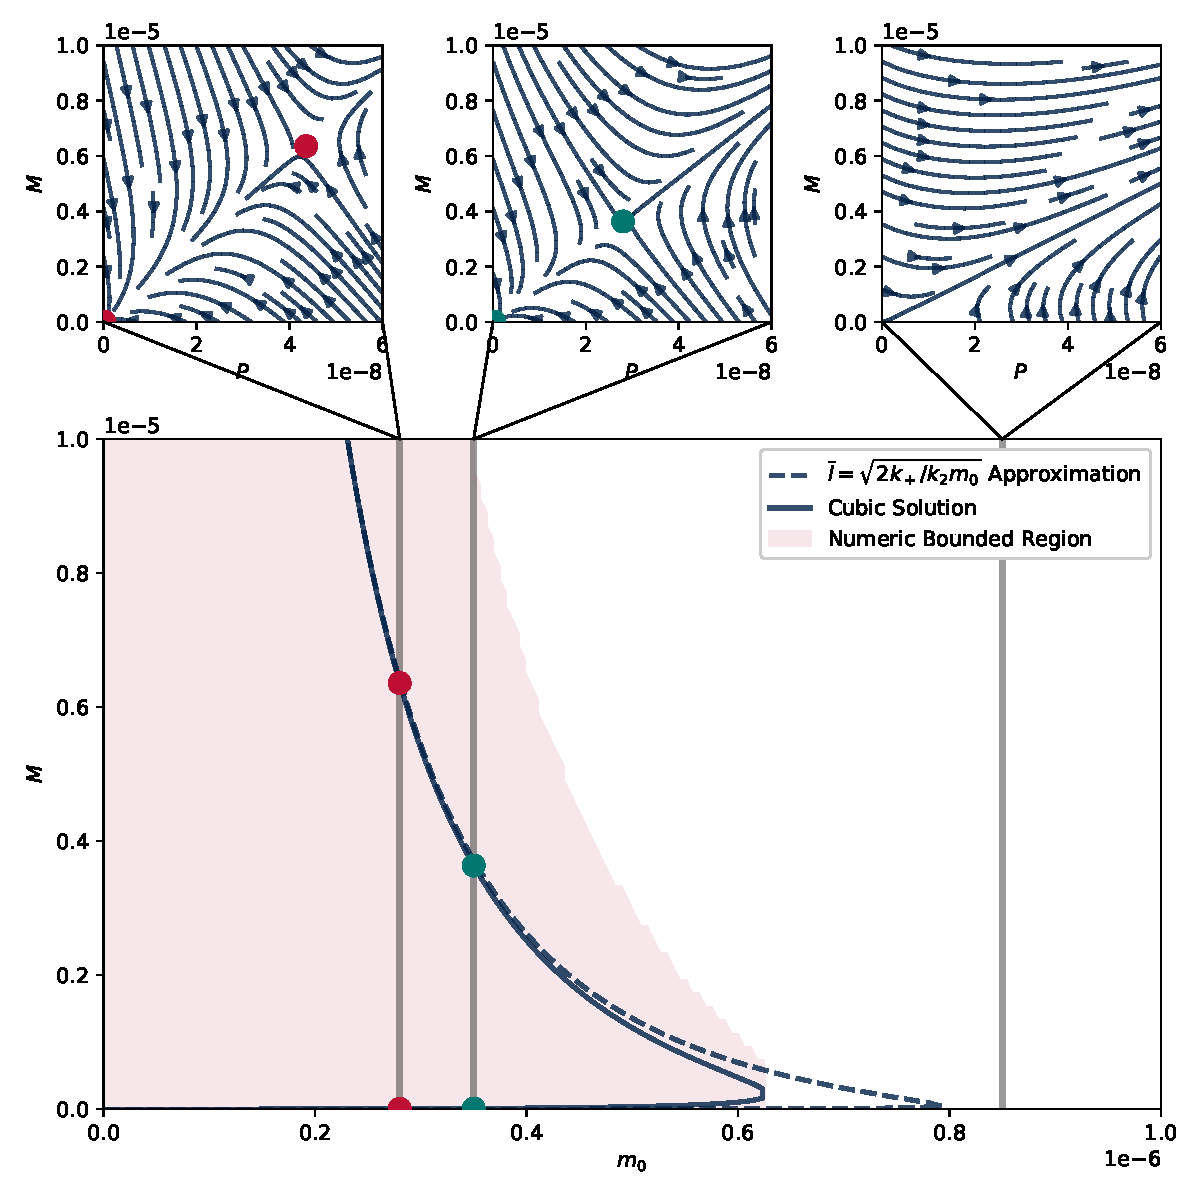
\includegraphics[width=0.8\textwidth]{figures/4-agg-figs/confusingNumericRegion.pdf}
    \caption{Comparison of the different descriptions of the system, its flow and stability.}
    \label{fig:4-steadyMM}
\end{figure}

\subsection{Reduced Models of in vivo Aggregation}

When the aggregate clearance and other rates are prescribed, the system and its dynamics are determined by three variables, $M$, $P$ and $m_0$, where $m_0$ is unaffected by the aggregation kinetics, however we keep this as a system variable to explore the role of monomer reducing therapies.

\subsubsection{Constant Clearance}

The fate of a system determines whether a cell is \textit{healthy} or \textit{diseased} with unbound growth describing the diseased state and a finite steady state for healthy cells. In the three parameter description, this will be entirely determined by the monomer concentration. We can further reduce the system to a two parameter description by prescribing the average length of the aggregates, $\bar{l}$. In the case of unbound proportional clearance, the steady state is given by $\mathbf{q}=\mathbf{A}^{-1}\mathbf{b}$ and so an obvious choice for $\bar{l}$ is to choose the steady state value, $\bar{l}^*=M^*/P^*$, equation (\ref{eq:4-lbarConstClear}), which exactly recovers the same steady state mass ($M^*$) as the full model. With this assumption, the moment equation for $M$ becomes
\begin{equation}
    \frac{\text{d}M}{\text{d}t}= \nc k_n m_0^{\nc} + n_2 k_2 m_0^{n_2} M + 2 k_\text{on} m_0 M/\bar{l}^* - \lambda M.
    \label{eq:4-reducedConstClear}
\end{equation}
Along with $\text{d}m_0/\text{d}t=0$ this defines a reduced model that captures the key features of the aggregation kinetics: the approach to the steady state for $m_0 < m_0^{\text{crit}}$ and unbound growth for $m_0 > m_0^{\text{crit}}$. A phase plane of this model clearly shows the dynamics and the emergence of the stability. When the aggregate mass is very low, the mass increases (flows upwards on the plot) until it approaches the steady state line and is balanced by clearance. When the monomer concentration is high ($m_0>m_0^{\text{crit}}$) there is no steady state distribution and so the aggregate mass will continue to increase. When the monomer concentration is low ($m_0<m_0^{\text{crit}}$) and the mass of aggregates is high, aggregates will be cleared from the system (move down on the phase plane) until the system reaches the steady state mass concentration.

% \begin{figure}
%     \centering
%     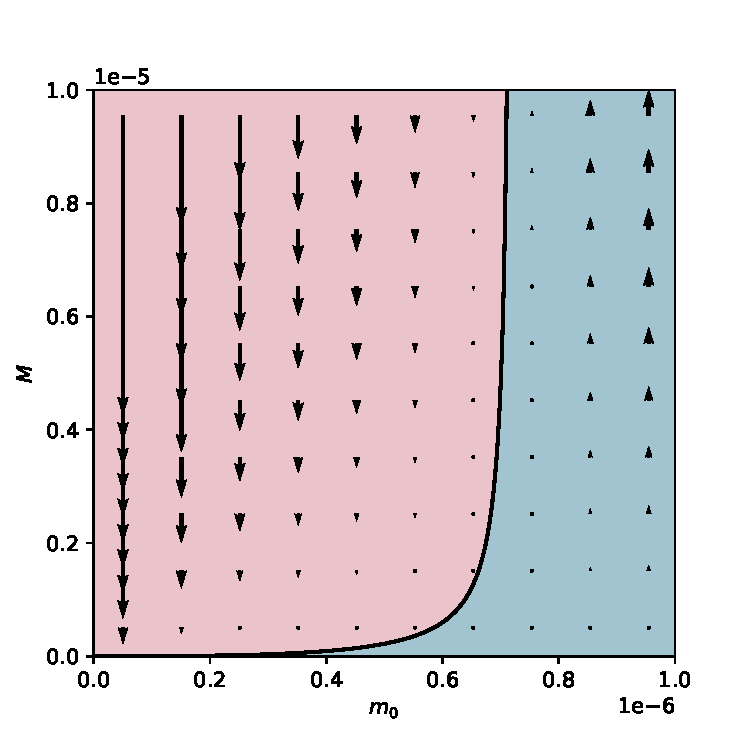
\includegraphics[width=0.8\textwidth]{figures/4-agg-figs/flowConstClear_nocol.pdf}
%     \caption{Flow for const clear.}
%     \label{fig:4-flowConstClear}
% \end{figure}
The average length assumption projects the two dimensional $M-P$ plane flows onto a line in $M-P$ space. Figure \todo{ref} shows this line and the key features of the dynamics are well captured by the projection onto the line. We assumed a linear relationship between $M$ and $P$, however a more complex functional relationship may capture the dynamics more accurately as there appears to an obvious slow manifold in the $M-P$ space, however the linear relationship captures the key features and makes it easy to interpret fixed points and their stability.

When the monomer concentration is high and the linear system grows unbound, the long time behaviour of $\mathbf{q}$ is determined by the eigenvector of $\mathbf{A}$ corresponding to the positive eigenvalue $\nu_+$. The ratio of the components of this eigenvalue gives the average length which is
\begin{equation}
    \bar{l} = \frac{m_0^{-\frac{n_2}{2}} \sqrt{k_2 n_2^2 m_0^{n_2}+8 k_\text{on} m_0}+\sqrt{k_2} n_2}{2 \sqrt{k_2}}.
\end{equation}
Typically, we expect $k_2 m_0^{n_2} \ll k_\text{on} m_0$ and thus $\bar{l} = m_0^{\frac{1-n_2}{2}}\sqrt{2 k_\text{on}/k_2}$. Using this $\bar{l}$ in the reduced dynamics, equation (\ref{eq:4-reducedConstClear}), predicts a much lower steady state mass (shown in Figure \ref{fig:4-steadyConstClear}), however both length distributions exactly capture the transition from the bound to unbound dynamics.
% The transition from unbounded growth to a finite steady state mass gives an expression for the critical clearance of a system. Alternatively, this transition can occur for a constant clearance that approaches a steady state if the monomer concentration is low, but grows unbound if the monomer concentration is high. Plotting the steady state mass, $M^*$, against the monomer concentration shows this transition. A system initialised with a total mass below the steady state mass, $M_0 < M^*$ will increase to $M^*$ and a system with $M_0 > M^*$ will decrease to $M^*$. When $M^*$ does not exist then the mass increasess without bound. To visualise this we assume that the number concentration is enslaved to the mass distribution, to give $P=M/\bar{l}$ even when the system has not equilibrated. This reduces the dynamics to be a function of $M$ and $m_0$ only and gives a two-dimensional phase plane of the system in this space and visualise the flows, as show in \todo{figure}. The app
\begin{figure}
    \centering
    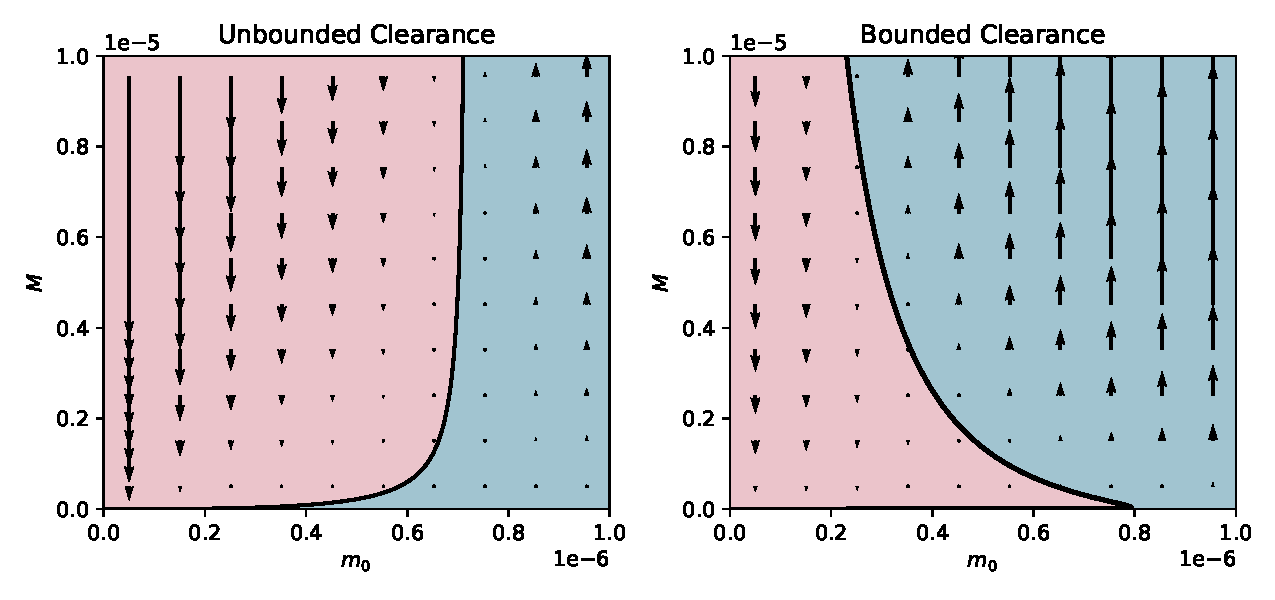
\includegraphics[width=0.95\textwidth]{figures/4-agg-figs/reduced_nocol.pdf}
    \caption{Flow for MM P.}
    \label{fig:4-flowMM_P}
\end{figure}

\subsubsection{Bound Clearance}

Similarly for the case of a bounded clearance, we reduce the model to a two parameter description by assuming a value of the  $\bar{l} = \sqrt{2 k_\text{on}/k_2 m_0}$ and $P=M/\bar{l}$.\todo{this is the eigenvalue of the exponentially growing mode!} The fixed points of this reduced system are now quadratic in $M$ and this gives two steady states when $m_0$ is low and no steady states when $m_0$ is high. This reduced model captures the key features of the full model, with the existence of a stable and unstable fixed point and a critical monomer concentration. However, the exact value at which this bifurcation occurs is different in the full and reduced models. This is due to the approximation for $\bar{l}$ being accurate for large steady state mass is large, which is the upper branch of the stability line at low monomer concentration. Fig \todo{which fig} shows that the two models agree in this region.

The fate of the system now depends on both the monomer concentration and the aggregate mass. The system is only stable, and therefore healthy, if both the monomer concentration and aggregate mass is low. Intuitively this dependence on the aggregate mass makes sense. If there are more aggregates (number and mass) in the system, then the rates of secondary nucleation and elongation will increase. When the aggregate clearance rate is high enough to out compete these effects then the aggregate mass/number is reduced and approaches a steady state value where the production of aggregates and clearance rates are balanced. For very large aggregate mass/number, the production rates of aggregates continue to increase with increasing aggregate mass/number, however for physically realistic models of clearance mechanisms the removal rate of aggregates will begin to saturate and at some point will no longer be able to balance the aggregate production/elongation rates, leading to runaway aggregation.

% \begin{figure}
%     \centering
%     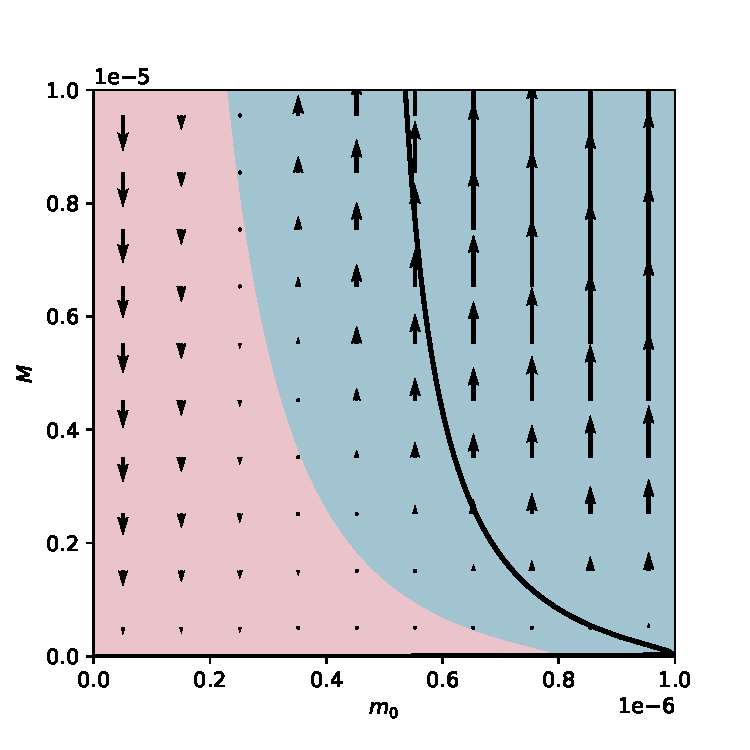
\includegraphics[width=0.8\textwidth]{figures/4-agg-figs/flowMM_nocol.pdf}
%     \caption{Flow for MM P.}
%     \label{fig:4-flowMM_P}
% \end{figure}

\section{Generalising the Dynamics}

\subsection{Generalised Models of Clearance}

When developing the model of bounded clearance in section \ref{subsec:4-boundedclearance} we focused on the kinetics of an enzyme-like mediated clearance mechanisms with binding rates independent of aggregate size. Crucially, this model predicts an upper unstable branch in the phase plane of the $M-m_0$ dynamics. However, this phenomena is general to any clearance that increases sub linearly with increasing aggregates. Since the aggregate production rate from nucleation is proportional to the mass of aggregates, any sub linear clearance will not be able to compete at large aggregate mass concentrations. For example, if the intermediary clearance component ($E$) can attach to aggregates at any position, then we would expect this binding rate to be proportional to the aggregate length and the dissociation to be remain constant, so that ${k_i^b}/{k_i^d}\sim i$. It also makes sense that the clearance processes, such as those from the proteasome system, will breakdown aggregates at a rate proportional to the number of monomer-monomer bonds that have have to be broken, $\sim(i-1)$, and so we can approximate $k_i^{c} \sim i^{-1}$. With these modifications, the clearance rate now saturates in $M$, rather than $P$ giving clearance for the number and mass concentrations as $\Tilde{\lambda}P/(\Tilde{K}+M)$ and $\Tilde{\lambda}M/(\Tilde{K}+M)$ respectively. When the rate constants $\Tilde{\lambda}$ and $(\Tilde{K})$ are scaled by a constant of the order of the average length, the system has identical behaviour to the number saturating clearance, although the exact fixed points are slightly perturbed. The reduced dynamics for this model is shown in the first panel of Figure \ref{fig:4-generalReduced}.

We expect that the complex regulation of living systems will result in multiple mechanism to remove aggregates, with different kinetics and saturation. Again as long as the removal mechanisms are sublinear in mass, then the upper unstable branch mass will be bistable and the key features of the model remain. For example, combining a clearance proportional to mass and an MM-like clearance that saturates in aggregate number (the clearance mechanisms in equations (\ref{eq:4-reducedConstClear}) and(\ref{eq:4-reducedMM})) we find that the bifurcation point moves to a higher monomer concentration, but that the bifurcation structure remains almost unchanged, as can be seen in \todo{one of the panels} of Figure \ref{fig:4-generalReduced}.

\begin{figure}
    \centering
    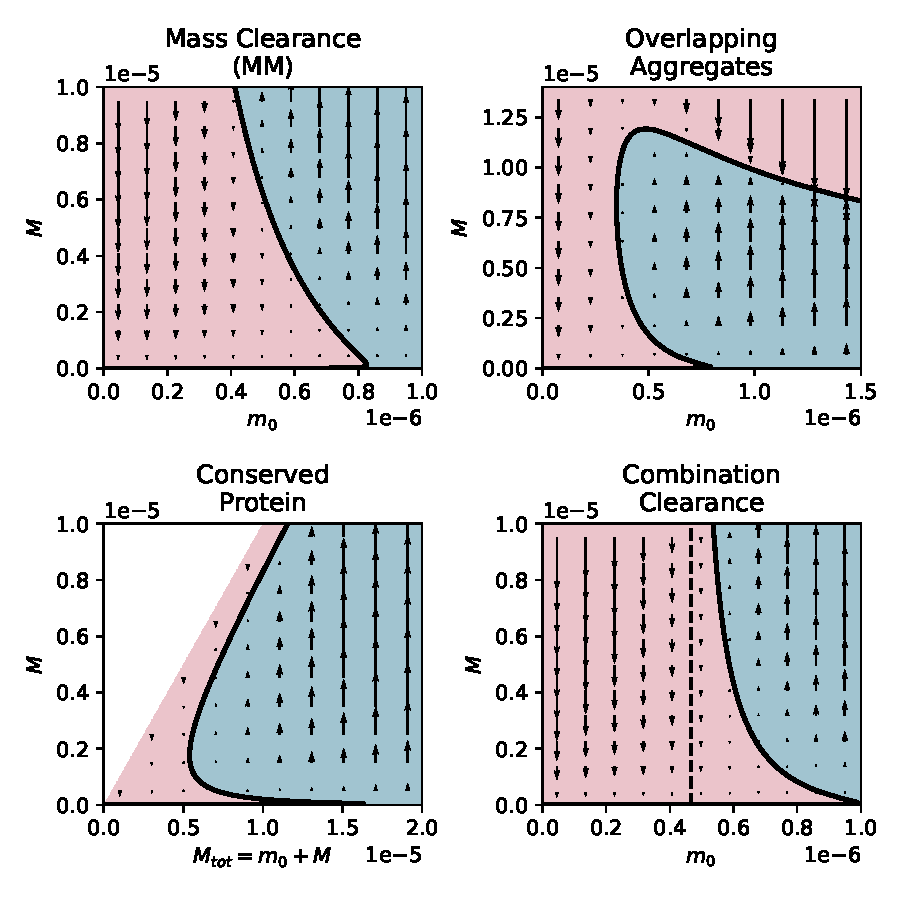
\includegraphics[width=0.95\textwidth]{figures/4-agg-figs/generalisingReduced_nocol.pdf}
    \caption{General reduced dynamics.}
    \label{fig:4-generalReduced}
\end{figure}

\subsection{Exponential Growth is Unphysical}

The exponential growth of the aggregate mass is labelled as the disease state. For a cell of finite volume and resources the exponential growth can only occur for finite time before other factors reduce the rate of growth. To describe this, we can modify the reduced model in equation \ref{eq:4-reducedMM} and introduce a correction to the secondary nucleation. As the aggregate concentration increases, multiple aggregates may touch or overlap in space and thus prevent this overlapping region of the aggregate surface from acting as a catalyst for secondary nucleation. We expect the overlapping region to increase like $M^2$ and so the aggregation kinetics with this corrected aggregate surface becomes
\begin{equation}
\frac{\text{d}M}{\text{d}t}= \nc k_n m_0^{\nc} + n_2 k_2 m_0^{n_2} (M- \rho M^2) + 2 k_\text{on} m_0 M/\bar{l} - \frac{\lambda_M M}{K_M+M/\bar{l}}
\end{equation}
where $\rho$ is the overlap constant. Figure \ref{fig:4-generalReduced} \todo{some panel} shows the reduced dynamics as before, however there is now a hysteresis loop. For very low monomer concentration there is only one steady state as the clearance mechanisms grow faster than the secondary nucleation and the steady state is determined by the balance of primary nucleation and clearance. For intermediate monomer concentrations, there is a region where the secondary nucleation dominates, as before, however additionally for larger aggregate mass the crowding effects prevent further increase in aggregate mass and there is a third steady state that is stable with large aggregate mass. For even larger values of aggregate mass, the system undergoes the same bifurcation as before for low values of the aggregate mass, but this large aggregate mass steady state persists and is attracting everywhere. Phenomenological, we interpret this exactly as before, however now the aggregate mass in the diseased state is bound at some very high aggregate mass, which is more physical. Despite being bound, we expect that this large aggregate mass will still be toxic and thus is associated with the same pathology.


The models of aggregation considered so far assume constant monomer concentration in the cell, motivated by cellular homeostasis maintaining regulating this concentration. When the aggregate mass is large in the system the rate of aggregation will become increasingly fast and at some point will be on the same timescales as the regulation of monomer and so we cannot model the monomer as constant. An alternative is to assume the aggregation kinetics are much faster than the expression of the monomer and so the total protein in the system, $M_{tot} = M + m_0$ is constant. Assuming the MM-like clearance mechanism, the rate of change of aggregate mass is still given by equation (\ref{eq:4-reducedMM}) and substituting $m_0=M_{tot}-M$, so that $\dot{M}=-\dot{m_0}$. Physically, this corresponds to clearance mechanisms converting the aggregated mass back into monomer to conserve total protein. The dynamics of the new reduced model can be seen in a phase plane of $M$ and $M_{tot}$, this is shown in \todo{a panel of} Figure \ref{fig:4-generalReduced}.

Since $\dot{M}=-\dot{m_0}$, the effects of the conserved total protein will be seen when the aggregate mass concentration is the same order of magnitude as the monomer concentration. \todo{actually, we should think about this a bit more} There is also a region of the graph that is unfeasible, corresponding to there being more aggregated protein than there is total protein, which is not possible.  We therefore chose rate constants that show the effects of the bounded clearance on a similar scale to the aggregate mass. From the plot it can be seen that system dynamics for conserved total protein has the similar structure as the saturating secondary nucleation, except with an increasing upper branch. The upper branch for large monomer concentration has almost all protein in the aggregated state, however there still exists some monomer so that the nucleation rates balance the clearance rates. As with the saturating secondary nucleation, the seeding, monomer dependence and effects of clearance are all phenomenological the same in this modified model compared to the original reduced model in equation (\ref{eq:4-reducedMM}).

This model and the model in equation (\ref{eq:4-reducedMM}) represent two distinct regimes: the aggregation kinetics are much fast than the homeostatic mechanisms or the inverse. The full system is likely to couple these timescales, and neither $\dot{m_0} \neq 0$ nor $\dot{M}_{tot} \neq 0$ so that the arrows in the reduced models will not longer be vertical, but will be tilted. It is harder to determine the fate of the system from the coupled dynamics, but looking the two limiting regimes we recover the same macroscopic behaviour consistent with seeding, monomer reduction therapies and the transitions to disease via reduced clearance.

\subsection{Length Dependent Seeding}

In coarse gaining the system dynamics to the $m_0-M$ space we ignored the dependence of the fate of the system on $P$. Looking at the top row of Figure \ref{fig:4-steadyMM}, we can see that for a constant initial mass, the number of aggregates can determine whether the system evolves to an unbound aggregate mass or the low aggregate mass steady state. In fact, there exists maximum number of aggregates for which the aggregates mass will remain bound and if there are initially more aggregates in the system than this, then the flow of the system will be towards the state of infinite aggregates. This result is useful to understand seeding experiments in vivo. An experimental challenge is to control the length distribution of aggregates that will be used to seed a system to investigate the in vivo dynamics. Here we see that a different length distribution can in fact alter the fate of identical cells and so conclusions drawn from comparing the aggregation kinetics with uncontrolled length distributions may be misleading.

\todo{actually this could be interesting because if, for example longer agregates diffuse more slowly, then overall number could become dependent... nice to connect to, for example Georgia's spreading? could think about extensions inspired by the kind of model in \cite{agudo-canalejo_cooperatively_2020}.}

\subsection{Length Dependent Clearance}

Another physically motivated modification to the constant clearance model is to reduce the rate of clearance for longer aggregates. We expect longer aggregates will take longer to clear from living cells and tissue as there are more bonds to break. It is useful to understand if this will recapitulate the observed seeding behaviour, that is, whether a sudden increase in the concentration of longer, more persistent fibrils would cause a transition to exponential growth. The logic of this argument is that since the longer aggregates take more time to clear, that by the time they are removed from the system, the increase in secondary nucleation and subsequent elongation will have already replenished and then increased the concentration of longer aggregates, leading to positive feedback.

As we expect the clearance to be proportional to number of bonds, which goes like aggregate length, we assume $\lambda_i = \lambda i^{nu} p_i$, where we choose $\nu=1$. For the non-fragmenting, non-depolymerising system discussed here, the master equation for this model 
\begin{equation}
    \frac{\text{d}p_i}{\text{d}t} = \delta_{i, n_C}k_n m^{n_C} + \delta_{i, n_2} k_2 m^{n_2} \left(\sum_{j=\nc}^{\infty} j p_j\right) + 2k_\text{on} m (p_{i-1}-p_i) - \lambda i^{-1} p_i.
    \label{eq:4-pi_evolution}
\end{equation}
Unlike the previous clearance models, summing over the aggregate population at each length introduces a dependence on the $-1^\text{th}$ moment, $Q^{-1}=\sum_i i^{-1}$, for the evolution of the aggregate number, $P$. This does not result in a closed moment equation that can be used to determine the transition to disease. Instead, we use the numeric solution to evolve the system for different initial values of $M$ and $m_0$. Figure \ref{fig:4-numinus1} shows the \todo{values tested} and shows the transition to stability for different values of $\lambda$. As can be seen from the plot, the system does not show a seeding-like transition to being unstable for increasing $M$ and the steady state dynamics are entirely determined by $m_0$.

This can be understood mathematically, since the evolution of all the $p_i$s define an infinite linear system, which can only support one steady state. If this steady state is positive then it will be attractive for all positive concentrations (since the primary nucleation always increases  $p_i$ as $p_i \to 0$). If it is not positive, then the concentration will increase unbound. \todo{Firm this up...} 

For $\nu=-1$ and using the approximation $Q^{-1}=P^2 / M$ gives
\begin{align}
    \frac{\text{d}M}{\text{d}t}&= \nc k_n m_0^{\nc} + n_2 k_2 m_0^{n_2} M + 2 k_\text{on} m_0 P - \lambda P \\
    \frac{\text{d}P}{\text{d}t}&= k_n m_0^{\nc} + k_2 m_0^{n_2} M - \lambda \frac{P^2}{M}.
    \label{eq:4-nudependent}
\end{align}
which we solve and for positive $M$ and $P$ to get
\begin{equation}
% k_2 \lambda^2 m_0^{n_2} - 4 k_2 k_\text{on} \lambda m_0^{1 + n_2} + 4 k_2 k_\text{on}^2 m_0^{2 + n_2} - k_2^2 \lambda m_0^{2 n_2} n_2^2 = 0
k_2 \lambda^2 - 4 k_2 k_\text{on} \lambda m_0 + 4 k_2 k_\text{on}^2 m_0^{2} - k_2^2 \lambda m_0^{n_2} n_2^2 = 0
\end{equation}
and we also require $\lambda - 2 k_\text{on} m_0 > 0$ which for $n_2 = 0$
\begin{equation}
m_0 = \frac{2 k_\text{on} \pm \sqrt{k_2\lambda} n_2}{4 \lambda^{-1} k_\text{on}^2 - k_2 n_2^2}
\end{equation}
reduced model works really well here! just set the $P=M/lbar$ with thee lbar from before!

\begin{figure}
    \centering
    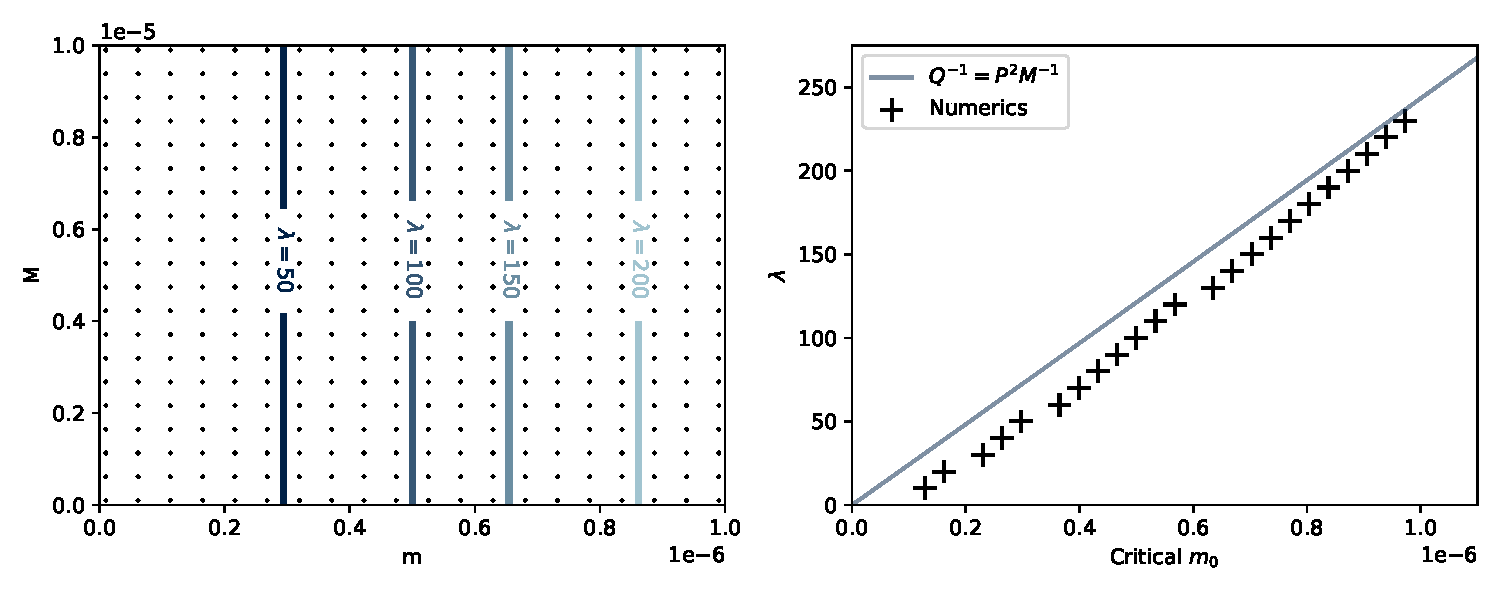
\includegraphics[width=0.9\textwidth]{figures/4-agg-figs/numinus1sidebyside.pdf}
    \caption{Length Dependent Clearance}
    \label{fig:4-numinus1}
\end{figure}

\section{Transitions to Disease and Therapeutic Scenarios}

The reduced model of the aggregation kinetics provides a powerful framework to unify experimental observations and to discuss key features of the the transition to the disease. In both of the reduced models and generalisations (plotted in Figs. (\ref{fig:4-flowConstClear}), (\ref{fig:4-flowMM_P}) and  (\ref{fig:4-generalReduced}) below) there exists a boundary in the $M-m_0$ space that separates systems that will undergo unbound aggregation and those that will have a long term finite aggregate mass. In samples from autopsies, diseased tissue contains cells that are saturated with aggregates. In our model the diseased cells correspond to unbounded aggregation and thus the onset of the disease corresponds to crossing this boundary. \todo{how many cells aggregated etc.} \todo{At some point should I include the exponential proliferation plot?} Each cell in a brain region will likely have different exact physical conditions that may cause slight variations between the exact reaction rates, clearance parameters and monomer concentrations. For example, spatial proximity to blood vessels or the lymphatic system might affect clearance mechanisms, the exact pressure of the internal cellular environment will affect reaction rates and cell-to-cell variability in gene expression will cause the monomer concentrations in different cells to vary \todo{are these good examples + references}. This variability means that each cell will have a slightly different stability line in the $M-m_0$ space. If the system parameters change slightly, then some of the cells may cross the stability line and transition into the unbound aggregation state and ultimately trigger the disease.

\subsection{Ageing reduces Clearance}
\cite{keller_decreased_2000}
A cell in the healthy state can transition to a diseased state if the rate of in vivo clearance mechanisms reduce. For example ageing, or other long term stress on the immune system, might reduce the concentration of the intermediary clearance species, or blood flow in the brain, corresponding to a reduction in the saturating clearance rate, $\lambda_M$ in the model in equation (\ref{eq:4-reducedMM}). This moves the critical line and in particular the value of the monomer concentration at which the bifurcation occurs, $m_0^{(crit)}$. A previously healthy cell with monomer concentration greater than the new critical value, $m_0 > m_0^{(crit)}$, will have transitioned into the disease state and will accumulate aggregates.

The delay before this transition occurs depends on the value of $m_0$ of a cell and how close that is to the initial bifurcation point, $m_0^{(crit)}$ as well as the rate of clearance decline. Individuals with genetic disorders that increase $m_0$ show an earlier onset of disease \todo{ref and discuss more} and impact from sports of other vocations which we expect to reduce clearance more rapidly also show a younger onset of disease \todo{ref and discuss more}.

\subsection{Explaining Genetic Susceptibility}

AD has a high heritability, suggesting there is a genetic component that can cause predisposition to development of the disease in a wide range of adults \cite{bellenguez_genetics_2020}. Genome-wide association studies correlate AD with a variety of gene sets, with the main implications being associations with amyloid/tau and microglia \cite{bellenguez_new_2022}. As discussed, changes in the quantity and quality of monomer protein expression can increase susceptibility to disease. The microglia are cells that support immune function and endocytosis with the brain, directly affecting the clearance mechanisms. These genetic studies do not provide mechanistic insight into the causes of disease, but rather suggest where to look. It is encouraging that two major features that determined the transition to disease in the model developed here, the monomer concentration and clearance mechanisms, were also identified as risk factors in human populations. Despite this currently being a very broad association, quantifying the rate parameters and the effects of mutations will hopefully make major strides towards understand and preventing the onset of the disease in humans.

AD has a reported higher prevalence in individuals with Down Syndrome (DS) \cite{head_aging_2012, zigman_alzheimers_2007}. Although harder to diagnose due to other \todo{impairements}, upto $55\%$ of DS adults aged 40-49 years may be clinically demented and almost all adults with DS over the age of 40 years have neuropatholigcal changes, for example $\beta$-amyloid (A$\beta$) \todo{AB vs BA?} plaques and neurofibrillary tangles, that would lead to a diagnosis of AD \cite{zigman_alzheimers_2007}. AD is more prevalent and has an earlier onset in adults with DS (for comparison see Section \ref{subsubsec:onsetage}). Alongside affecting immune responses, the additional copy of chromosome 21 (which is the genetic basis of DS) increases the expression of amyloid precursor protein \cite{head_aging_2012, rumble_amyloid_1989}. The gene coding for amyloid precursor protein is on the long arm of chromosome 21 and so the trisomy can lead to overexpression of this gene and an increased concentration of the aggregating monomer. However, the mechanistic cause of this correlation has not been understood previously. This work gives a mechanistic grounding that explains the early age of AD onset in adults with DS. The increased protein expression moves the cells and tissues closer to the critical point  in Figure \ref{fig:4-flowMM_P}. As such, a smaller reduction in the clearance rate can trigger the transition to disease, resulting in an earlier age of onset.

\subsection{Rational Therapeutic Design}

\todo{Discuss currently available therapeutics}

In addition to explaining the onset of disease, understanding the mechanisms governing neurodegenerative diseases is essential in the rational design of therapeutics. In the kinetic framework discussed here, an effective therapy will transition cells or tissues from the unstable to stable regions and ensure the stability of the aggregate mass in the future.

\begin{figure}
    \centering
    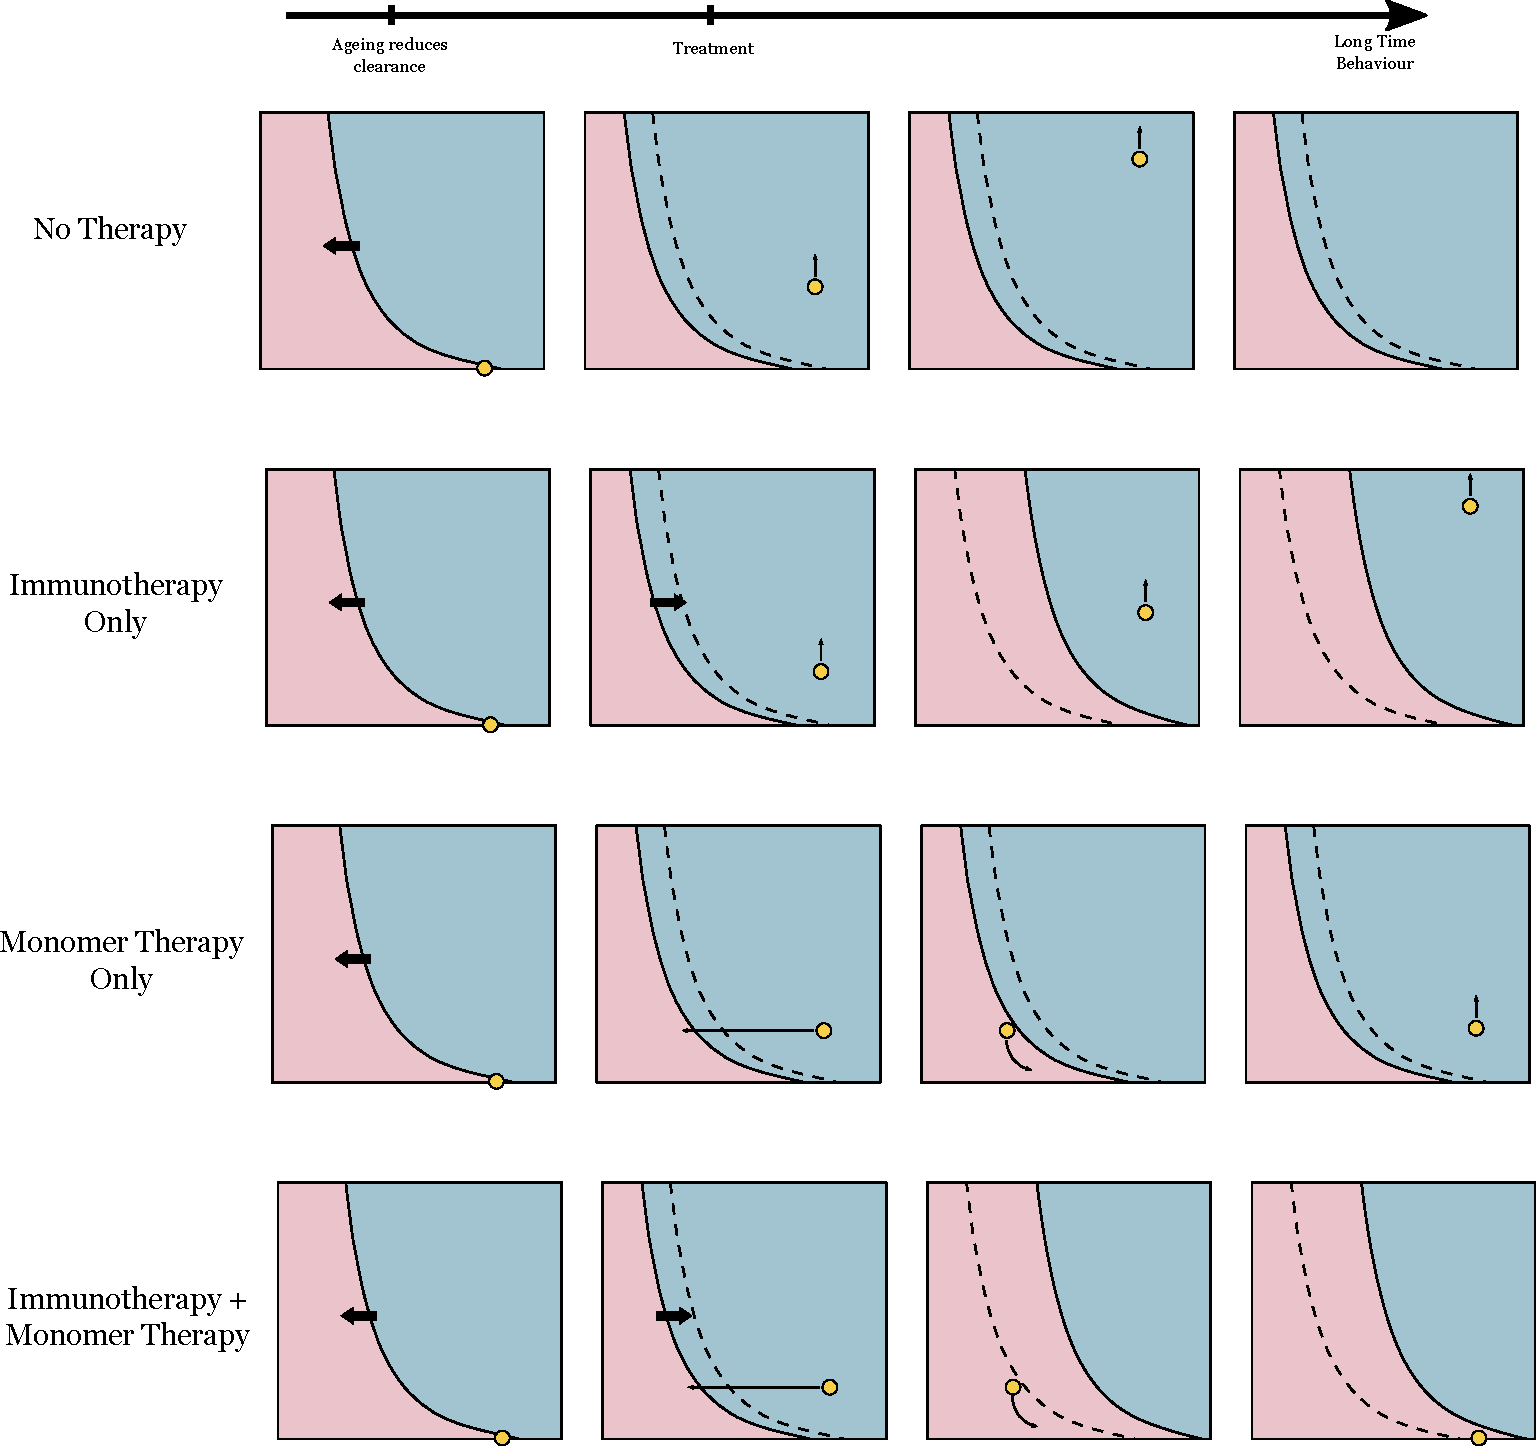
\includegraphics[width=0.9\textwidth]{figures/4-agg-figs/therapyScheme.pdf}
    \caption{Examples of therapeutic schemes.}
    \label{fig:4-therapyscheme}
\end{figure}

The immunotherapy treatments currently under development focus on increasing the clearance mechanisms in the brain. This will shift the balance of aggregation and removal, moving the transition boundary and increasing the area of the stable region. However, since the system will begin proliferating aggregates as soon as it becomes unstable, then the efficacy of the response will depend on how soon any intervention is made after the system become unstable. At early times after the transition, the system will still be close to the stable region, however at later times after more aggregation it will be further from the transition boundary so that the increased clearance does not return the system to being stable. This situation is shown in the second row of Figure \ref{fig:4-therapyscheme}. The best time to take immunotherapy treatments would be before the transition to the unstable region, however it is hard to identify exactly when individuals would become at risk and so hard to design a resource effective treatment strategy at the population level. Furthermore, increasing the population taking medication that may not as susceptible to the onset of disease will also alter the calculation of risks associate side effects of the treatment.

An alternative therapeutic strategy is to develop monomer-reducing therapies, for example ASO-like treatments, or \todo{CHARM system?}. Reducing the monomer concentration can cause an unstable system to cross the transition boundary and return to being stable. The aggregates will then be cleared more quickly than they are produced and the aggregate mass will return to the low stable concentration. However, after some time, the effects of the monomer therapy will reduce and the monomer concentration will return to its original value, once again transitioning into the unstable region so that the aggregates proliferate. This situation is shown in the third row of Figure \ref{fig:4-therapyscheme}. Repeated monomer therapies that act to keep the monomer concentration at some reduced value could keep the system stable, however repeated exposure to ASOs can become toxic \todo{etc etc} and if the protein monomer is functional then reducing its concentration could affect the healthy function of the cell.

An alternative therapeutic strategy that this theory predicts could be a combination therapy of both immunotherapy and monomer reducing therapy. Reducing the monomer ensures an initial transition to the stable region and the subsequent immunotherapy ensures that the system remains in this stable region in the longer term. The final row of Figure \ref{fig:4-therapyscheme} demonstrates how this process will lead to longer term stability. This type of combination therapy would overcome the challenges associated each treatement indivudally, however the exact \todo{need to know the exact sizes of effects etc.}

\section{Summary and Conclusions}


oligomeric proteins reduce transit time between by dissassembling, diffuse more quickly and then reasssembling \cite{agudo-canalejo_cooperatively_2020}

This chapter presents a theory for the kinetics of neurodegenerative diseases that can explain different aspects of the disease into one unified theory. This combines all existing phenomena into one model that 

Unfieid theory, difference regions for different diseases

Could be oligomers that actually cause the disease, but as shown in the first few sections aggregates of all lengths will increase together linearly.

If a lot of small aggregates spread, disease can be triggered below the transition mass -> an argument around the spreading dynamics.

The real need now is to get the parameters in vivo. Talk about randalls data and the fact that time coursing will reveal the role of the two state transition vs stochastic limited nucleation limited aggregation.